\problemname{}

Emilia and her brother Alex meet up with a lot of friends in the park to play table tennis together.
Since there is only one table, they play round-the-table which is everybody's favourite.

The rules are simple:
There are $\ell \geq 2$ kids queueing up on the left side and $r \geq 1$ kids queueing up on the right side of the table.
The first kid on the left side starts with the ball.
Whoever has the ball hits it over the net onto the opposite side and runs around the table to join the queue at the opposite side.
This is repeated until the first mistake.

\begin{figure}[h]
	\centering
	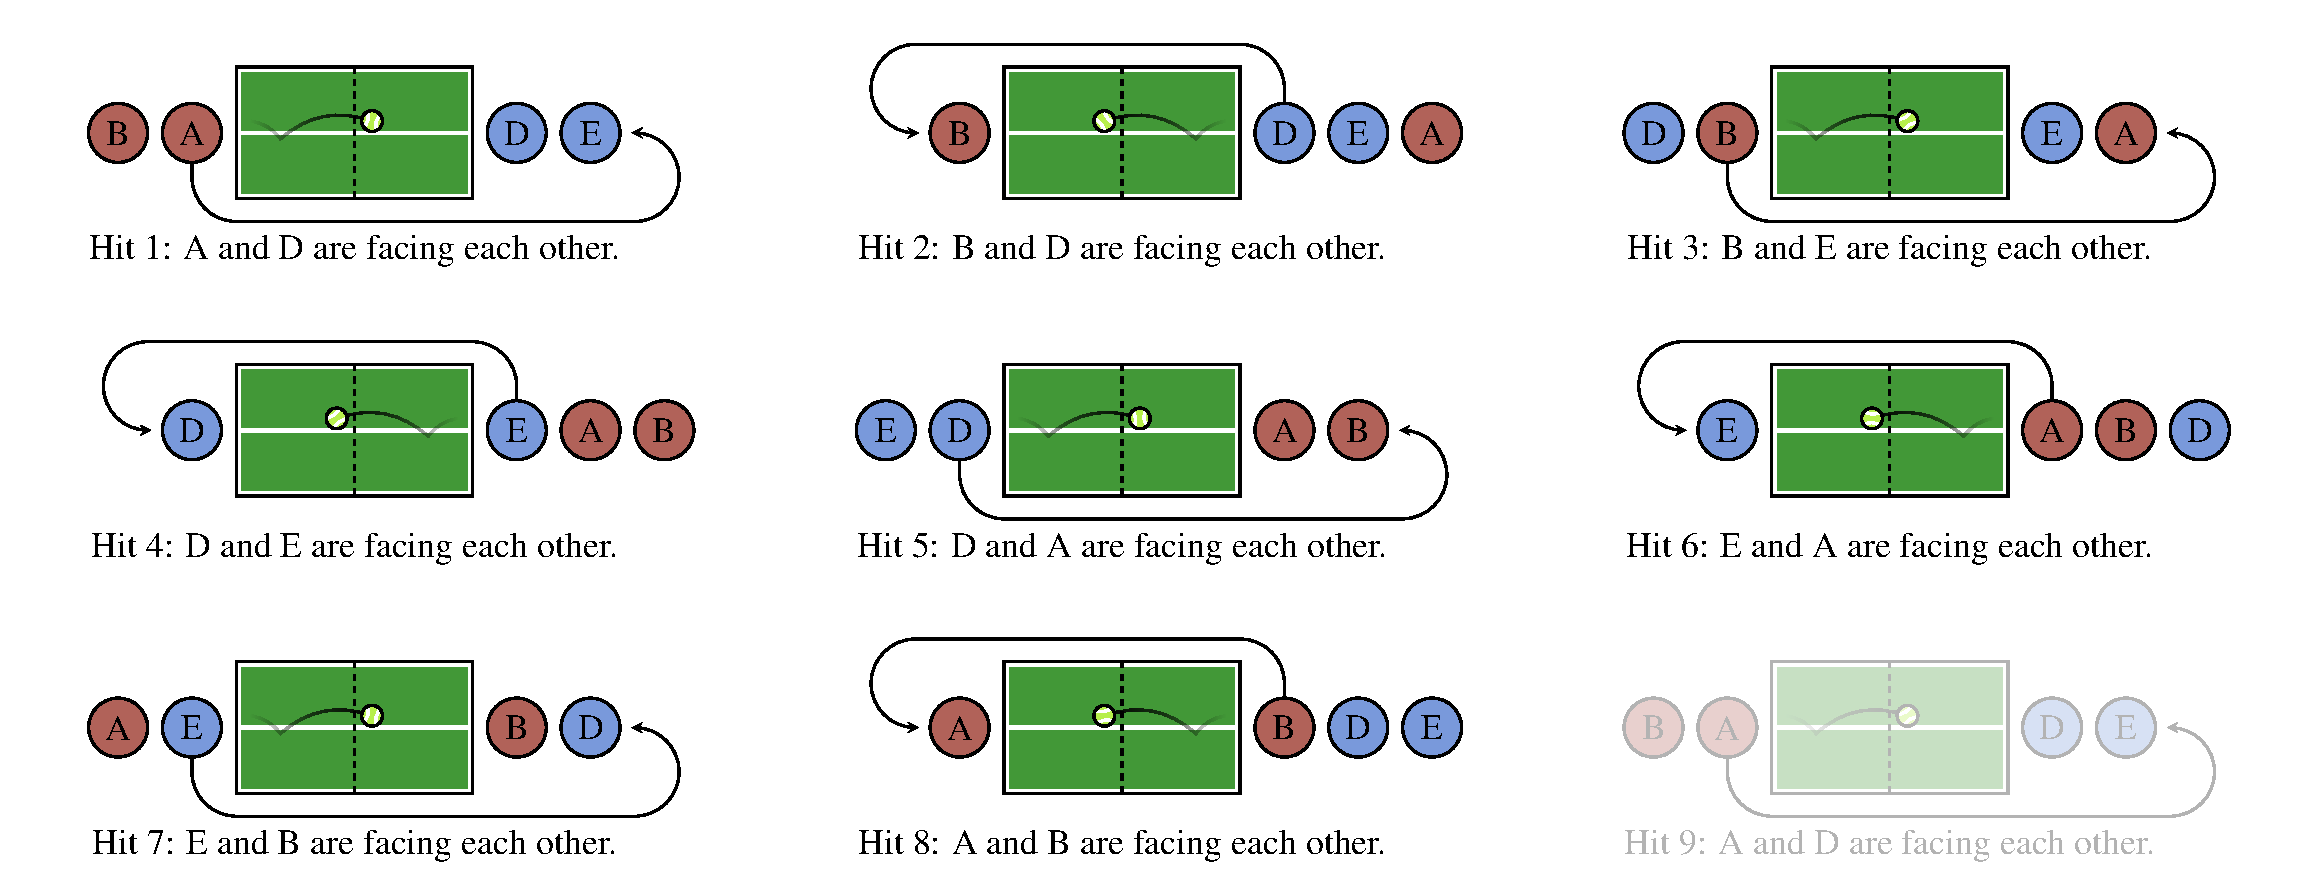
\includegraphics[width=\textwidth]{sample}
	\caption{Visualization of the first sample.
		During Hit~$1$ and $5$, and during Hit~$3$ and $7$, we observe the same pairing.
		After $8$ hits we end up in the initial state again and cannot observe any new pairing afterwards.
		Therefore, there are $6$ different pairings we will see in total.
	}
\end{figure}

Emilia, Alex, and their friends play this game all the time and are so good that they can go on almost forever without making any mistake.
After some time, Emilia notices that she has never faced Alex, meaning that they have never been at the front of opposite queues at the same time.
She wonders if this will ever happen in this round.
Curious about this, she starts keeping track which pairings have already faced each other.

How many different pairings has she counted after the ball went over the net $10^{10^{100}}$ times?

\begin{Input}
	The input consist of:
	\begin{itemize}
		\item One line with two integers $\ell$ and $r$ ($2 \leq \ell \leq 10^{9}$ and $1 \leq r \leq 10^{9}$), the number of players on the left and right side of the table, respectively.
	\end{itemize}
\end{Input}

\begin{Output}
	Output the number of different pairings Emilia counts.
\end{Output}
